\section {Descripción general del producto}
	El producto que se desea fabricar es una mesa de billar. En particular una mesa de \emph{pool}.
El producto esta formado por una  mesa con un tablero de pizarra forrada de paño, rodeada de bandas de material elástico y con seis troneras. 
	
	\subsection {Utilidad y aplicaciones}
	La mesa de billar es usada para la práctica de un deporte llamado billar. Este deporte olimpico desde el 2004, tubos sus inicios en la 
 antigua  Grecia y Egipto, pero es en la Europa del siglo XV cuando se empezo a tomar la forma del juego que se conoce en la actualidad. 

El billas consiste en: impulsar un número variable de bolas con la ayuda de un taco,  el cual lleva adosado en su extremo anterior una suela de cuero.
Con este movimiento debemos procurar introducir unas bolas (de materiales sintéticos con cualidades elásticas similares a las del marfil) dentro de las troneras.

	\subsection {Mercado}

El mercado de este productos suele abarcarlo en casí su totalidad los locales de ocio,(bares y recreatibos...). Tambien hay particulares que desean obtener una
mesa de billar, pero debido a su coste elebado son pocos los que pueden permitirse tener una en sus hogares. 
    
\section {Diseño del producto}

	\subsection {Definición técnica (dimensiones, especificaciones técnicas)}
			\begin{enumerate}
			\item Las mediadas de la mesa de billar pueden bariar ligeramente siempre y cuando respetemos algunas medidas estandar. En este caso las medidas elejida para la mesa son:
				\begin{itemize}      
				\item Medidas del campo de juego del billar: 200 x100 cm.

				\item Medidas exteriores: 232 x 132 Altura: 80cm
				\end{itemize}
				

			\item La superficie de la mesa es una la losa de pizarra 20 mm. Recubierta de un fieltro(lana y nailon) berde de 600g.

			\item Los bordes del campo de juego en los que las bollas tienen que rebotar esta compuesto por (goma vulcanizada + lana)
			\end{enumerate}


	\subsection {Definición geométrica}
		    \begin{enumerate}
		     \item La superficie del juego debe ser reztangulas y poseer 6 abujeros por donde se introduciran las bollas de x cm. Lo  abujeros estaran distribuidos como
			    muestra la siguiente figura.
		     \item Los bordes del campo (goma) estan por todo el perimetro del campo salvo por donde hay abujeros y mide  3 cm de grosor.

		     \item Para la definizión geométrica de como son las demas piezas  se adjunta vistas que exlique mejor que con palabras que aparienzia tiene la mesas de billar
			  y sus diferentes elementos.
    			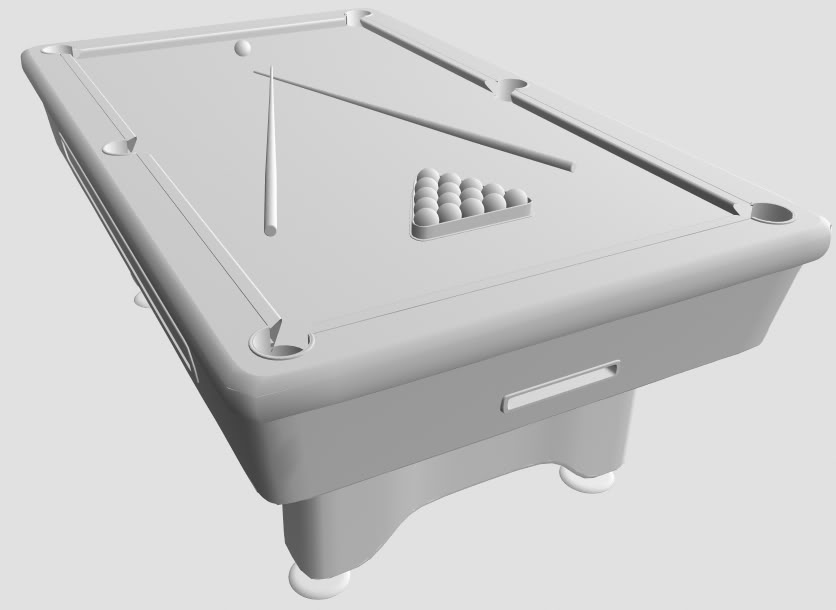
\includegraphics[width=0.8\textwidth]{prueba_billar.jpg}
			
		    \end{enumerate}


		    

	\subsection {Definición mecánica}
		    Cuando una bola cae a un abujero se pueden fabricar muchos y muy complejos mecanismos de recojida de la bola pero un mecanismo muy estendido,
		    fiable y muy empleado en las mesas de billar, que residen en las bibiendas, es poner unas troneras que guarden la bola una vez caida por el abujero hasta que queramos empezar
		    el juego de nuebo. Estas troneras o recipientes pueden ser de muchos materiales pero en nutro caso seran de plastico duro y lo sun ficientemente grandes como para quepan casi todas las bolas. 
\section {Fabricación del producto}

	\subsection {Recepción de piezas y/o materiales}

	\subsection {Proceso de fabricación detallado}

\section {Mercado}

	\subsection {Comercialización del producto}


\subsection{bibliografía}

%http://www.donbillar.com/mesas_de_billar.html

%http://www.youtube.com/watch?v=8cjHNDAokqs

%http://construyeloya.blogspot.com/2007/09/construye-tu-propia-mesa-de-billar.html

%http://www.construirmesadebillar.com/